\documentclass[10pt,a4paper]{article}
\usepackage[utf8]{inputenc}
\usepackage[portuguese]{babel}
\usepackage[T1]{fontenc}
\usepackage{amsmath}
\usepackage{amsfonts}
\usepackage{amssymb}
\usepackage{graphicx}
\usepackage[left=2.5cm,right=2.5cm,top=2.5cm,bottom=2.5cm]{geometry}
\usepackage{listings}
\usepackage{color} %red, green, blue, yellow, cyan, magenta, black, white
\definecolor{mygreen}{RGB}{28,172,0} % color values Red, Green, Blue
\definecolor{mylilas}{RGB}{170,55,241}

\author{Murilo Camargos}
\title{Métodos Computacionais - Aula 1}
\begin{document}
\lstset{extendedchars=true, inputencoding=latin1,literate=
{á}{{\'a}}1
{à}{{\`a}}1
{ã}{{\~a}}1
{â}{{\^a}}1
{é}{{\'e}}1
{ê}{{\^e}}1
{í}{{\'i}}1
{ó}{{\'o}}1
{õ}{{\~o}}1
{ú}{{\'u}}1
{ü}{{\"u}}1
{ç}{{\c{c}}}1}
\lstset{language=Matlab,%
    %basicstyle=\color{red},
    breaklines=true,%
    morekeywords={matlab2tikz},
    keywordstyle=\color{blue},%
    morekeywords=[2]{1}, keywordstyle=[2]{\color{black}},
    identifierstyle=\color{black},%
    stringstyle=\color{mylilas},
    commentstyle=\color{mygreen},%
    showstringspaces=false,%without this there will be a symbol in the places where there is a space
    numbers=left,%
    numberstyle={\tiny \color{black}},% size of the numbers
    numbersep=9pt, % this defines how far the numbers are from the text
    emph=[1]{for,end,break},emphstyle=[1]\color{red}, %some words to emphasise
    %emph=[2]{word1,word2}, emphstyle=[2]{style},
    extendedchars=true,
    inputencoding=latin1, 
}


	\section{Exercícios (23/11/2017)}
	Use o método de integração numérica de Runge-Kutta para obter a aproximação da solução dos seguintes problemas de Cauchy\\
	
	1. \[R'(t)=U(t), \hspace{0.3cm} U'(t)=\frac{35\left(P_v-P_l\right) - 7U(t)^2\left(5P_l+5\epsilon_l+4P_v+4\epsilon_v\right)}{7R(t)\left(5P_l+5\epsilon_l+P_v+\epsilon_v\right)}, \hspace{0.3cm} R(0)=1, \hspace{0.3cm} U(0)=0.0001\]
	
	2. \[R'(t)=U(t), \hspace{0.3cm} U'(t)=\frac{35\left(P_v-P_l\right) - 7U(t)^2\left(5P_l+5\epsilon_l+4P_v+4\epsilon_v\right)}{7R(t)\left(5P_l+5\epsilon_l+P_v+\epsilon_v\right)}, \hspace{0.3cm} R(0)=0.5, \hspace{0.3cm} U(0)=0.146446\]
	
	Adote os seguintes valores para os parâmetros: $P_v=0.166391$, $P_l=0.195091$, $\epsilon_v=1.79634$ e $\epsilon_l=4.34802$. Note que $U$ é a primeira derivada de R com relação a $t$.
	
	\section{Resolução}
	
	O método de Runge-Kutta foi implementado em MATLAB
	
	\subsection{Exercício 1}
	No exercício 1, o valor do passo escolhido foi $h=0.1$ e o intervalo de simulação foi definido como $t=[0,12.5]$, pois após este limite superior, o resultado iria pra infinito.    
    
    \begin{figure}[h!]
    \centering
      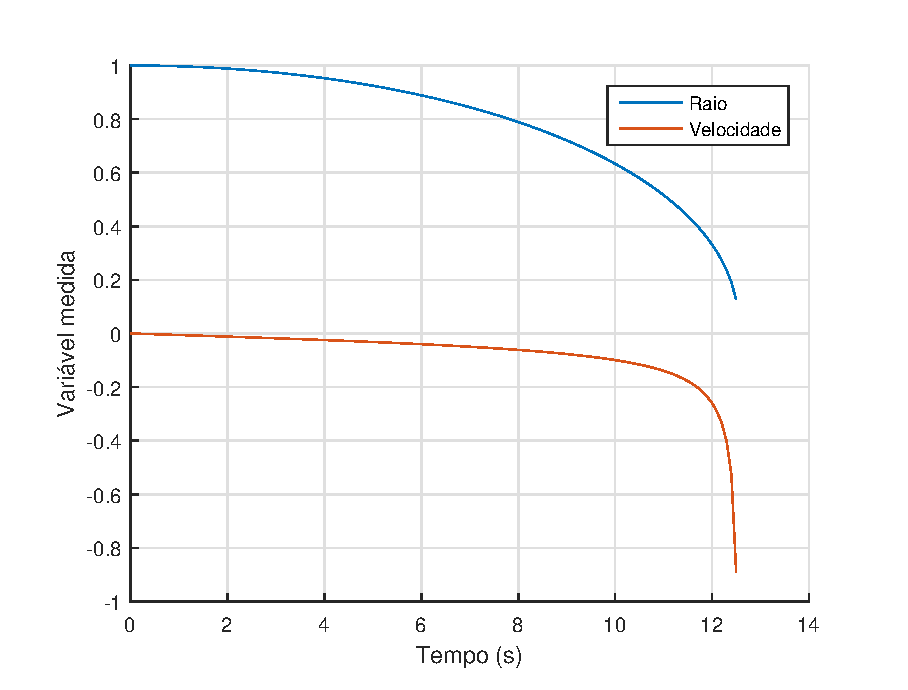
\includegraphics[width=0.8\linewidth]{figures/ex1h0-1t12-5.eps}
      \caption{Variáveis medidas no exercício 1.}
      \label{fig:ex1h0.1t12.5}
	\end{figure}
    
    \newpage
    \subsection{Exercício 2}
    
    No exercício 2, o valor do passo escolhido foi $h=0.2$ e o intervalo de simulação foi definido como $t=[0,22]$, pois após este limite superior, o resultado iria pra infinito.    
    
    \begin{figure}[h!]
    \centering
      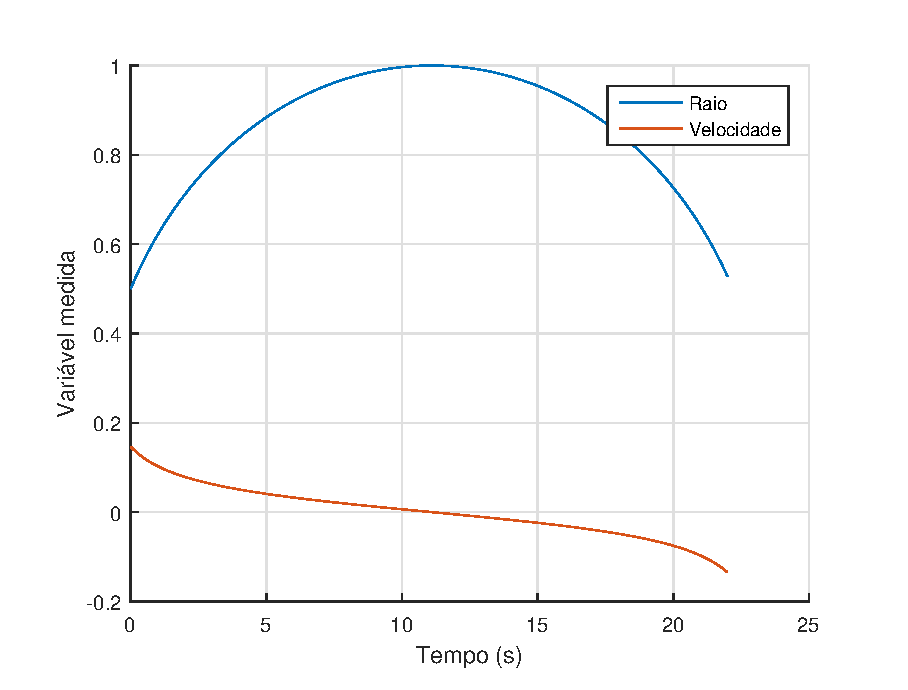
\includegraphics[width=0.8\linewidth]{figures/ex2h0-2t22.eps}
      \caption{Variáveis medidas no exercício 2.}
      \label{fig:ex1h0.1t12.5}
	\end{figure}
    
    \newpage
    \subsection{Código em MATLAB}
    \lstinputlisting[language=matlab]{code/bolha.m}
    \subsection{Runge-Kutta de quarta ordem}
    \lstinputlisting[language=matlab]{../tools/rk4.m}
    
\end{document}